\chapter{Monte Carlo Simulation}\label{cap:montecarlo}

The modern version of the Monte Carlo method was invented in the late
1940s by Stanislaw Ulam, while he was working on nuclear weapons
projects at the Los Alamos National Laboratory.
Monte Carlo methods, or Monte Carlo experiments, are a broad class of
computational algorithms that rely on repeated random sampling to obtain
numerical results. 

They are widely used in many fields: engineering,
physics, computational biology, computer graphics, applied statistics,
artificial intelligence for games, search and rescue and of course
finance and business.
In this Chapter we will review it and see some useful application to finance.

\section{The algorithm}\label{whats-monte-carlo-simulation}

The underlying concept to Monte Carlo simulation is to use randomness to solve
problems that might be deterministic in principle. It can be used to 
solve any problem
having a probabilistic interpretation since by the law of large numbers, the
expected value of some random variable ($Y$) can be approximated by taking the
empirical mean of independent samples of that variable:

\[ \hat{\mu}_n = \frac{1}{n}\sum_{i=1}^{n}{Y_i} \]

Three are the main classes of problems where it is applied: optimization, numerical
integration, and generating draws from a probability distribution.

Monte Carlo methods follow this particular pattern:
\begin{itemize}
\tightlist
\item
  define a domain of possible inputs;
\item
  generate inputs randomly from a probability distribution over the
  defined domain;
\item
  perform a deterministic computation on the generated inputs;
\item
  aggregate the results.
\end{itemize}
In the next Sections we will see each point applied to practical examples.

\section{Pseudo-Random Numbers}\label{pseudo-random-numbers}

The second point above implies that Monte Carlo methods require 
large amounts of random numbers to
generate the inputs, and it was their use that spurred the development
of pseudo-random number generators. 

Every programming language has libraries that
allows to produce huge series of random numbers (with a periodicity of
\(2^{19937}\)). These series are calculated by algorithms that take as
input a \emph{seed} which determines them uniquely. This means
that choosing the same seed you will produce the same set of numbers
every time (which is great for debugging purposes).

In \texttt{python} one of the available modules to generate random numbers is \texttt{random} which has, among others, the following useful functions:
\begin{itemize}
\tightlist
\item
  \texttt{seed} set the seed of the random number generator;
\item
  \texttt{random} returns a random number between 0 and 1 (with uniform
  probability);
\item
  \texttt{randint(min,\ max)} returns an integer random number between
  \texttt{min} and \texttt{max} (with uniform probability);
\item
  \texttt{sample(aList,\ k=n)} samples n elements from the list
  \texttt{aList}.
\end{itemize}
As usual for a more detailed description check \texttt{help(random)}.
The next example that shows an application of these functions besides the effect of  changing the seed of the random number generator.

\begin{tcolorbox}[breakable, size=fbox, boxrule=1pt, pad at break*=1mm,colback=cellbackground, colframe=cellborder]
\begin{Verbatim}[commandchars=\\\{\}]
\PY{k+kn}{import} \PY{n+nn}{random} 

\PY{n}{random}\PY{o}{.}\PY{n}{seed}\PY{p}{(}\PY{l+m+mi}{1}\PY{p}{)}
\PY{n+nb}{print} \PY{p}{(}\PY{l+s+s2}{\PYZdq{}}\PY{l+s+s2}{seed is 1}\PY{l+s+s2}{\PYZdq{}}\PY{p}{)}
\PY{n+nb}{print}\PY{p}{(}\PY{n}{random}\PY{o}{.}\PY{n}{random}\PY{p}{(}\PY{p}{)}\PY{p}{)}
\PY{n+nb}{print}\PY{p}{(}\PY{n}{random}\PY{o}{.}\PY{n}{random}\PY{p}{(}\PY{p}{)}\PY{p}{)}

\PY{n}{random}\PY{o}{.}\PY{n}{seed}\PY{p}{(}\PY{l+m+mi}{2}\PY{p}{)}
\PY{n+nb}{print} \PY{p}{(}\PY{l+s+s2}{\PYZdq{}}\PY{l+s+s2}{seed is 2}\PY{l+s+s2}{\PYZdq{}}\PY{p}{)}
\PY{n+nb}{print}\PY{p}{(}\PY{n}{random}\PY{o}{.}\PY{n}{random}\PY{p}{(}\PY{p}{)}\PY{p}{)}
\PY{n+nb}{print}\PY{p}{(}\PY{n}{random}\PY{o}{.}\PY{n}{random}\PY{p}{(}\PY{p}{)}\PY{p}{)}

\PY{n}{random}\PY{o}{.}\PY{n}{seed}\PY{p}{(}\PY{l+m+mi}{1}\PY{p}{)}
\PY{n+nb}{print} \PY{p}{(}\PY{l+s+s2}{\PYZdq{}}\PY{l+s+s2}{seed is 1 again}\PY{l+s+s2}{\PYZdq{}}\PY{p}{)}
\PY{n+nb}{print}\PY{p}{(}\PY{n}{random}\PY{o}{.}\PY{n}{random}\PY{p}{(}\PY{p}{)}\PY{p}{)}
\PY{n+nb}{print}\PY{p}{(}\PY{n}{random}\PY{o}{.}\PY{n}{random}\PY{p}{(}\PY{p}{)}\PY{p}{)}

\PY{n+nb}{print}\PY{p}{(}\PY{n}{random}\PY{o}{.}\PY{n}{randint}\PY{p}{(}\PY{l+m+mi}{1}\PY{p}{,} \PY{l+m+mi}{10}\PY{p}{)}\PY{p}{)}
\PY{n}{aList} \PY{o}{=} \PY{p}{[}\PY{l+s+s1}{\PYZsq{}}\PY{l+s+s1}{a}\PY{l+s+s1}{\PYZsq{}}\PY{p}{,} \PY{l+s+s1}{\PYZsq{}}\PY{l+s+s1}{b}\PY{l+s+s1}{\PYZsq{}}\PY{p}{,} \PY{l+s+s1}{\PYZsq{}}\PY{l+s+s1}{c}\PY{l+s+s1}{\PYZsq{}}\PY{p}{,} \PY{l+s+s1}{\PYZsq{}}\PY{l+s+s1}{d}\PY{l+s+s1}{\PYZsq{}}\PY{p}{,} \PY{l+s+s1}{\PYZsq{}}\PY{l+s+s1}{f}\PY{l+s+s1}{\PYZsq{}}\PY{p}{]}
\PY{n+nb}{print} \PY{p}{(}\PY{n}{random}\PY{o}{.}\PY{n}{sample}\PY{p}{(}\PY{n}{aList}\PY{p}{,} \PY{n}{k}\PY{o}{=}\PY{l+m+mi}{2}\PY{p}{)}\PY{p}{)}

seed is 1
0.13436424411240122
0.8474337369372327
seed is 2
0.9560342718892494
0.9478274870593494
seed is 1 again
0.13436424411240122
0.8474337369372327
2
['c', 'a']
    \end{Verbatim}
\end{tcolorbox}

The next lines of code shows instead how to draw a uniform distribution. Figure~\ref{fig:uniform_dist} shows the resulting distribution.

 \begin{tcolorbox}[breakable, size=fbox, boxrule=1pt, pad at break*=1mm,colback=cellbackground, colframe=cellborder]
\begin{Verbatim}[commandchars=\\\{\}]
\PY{n}{numbers} \PY{o}{=} \PY{p}{[}\PY{p}{]}
\PY{k}{for} \PY{n}{\PYZus{}} \PY{o+ow}{in} \PY{n+nb}{range}\PY{p}{(}\PY{l+m+mi}{10000}\PY{p}{)}\PY{p}{:}
  \PY{n}{numbers}\PY{o}{.}\PY{n}{append}\PY{p}{(}\PY{n}{random}\PY{o}{.}\PY{n}{randint}\PY{p}{(}\PY{l+m+mi}{0}\PY{p}{,} \PY{l+m+mi}{5}\PY{p}{)}\PY{p}{)}

\PY{k+kn}{from} \PY{n+nn}{matplotlib} \PY{k}{import} \PY{n}{pyplot} \PY{k}{as} \PY{n}{plt}
\PY{n}{plt}\PY{o}{.}\PY{n}{hist}\PY{p}{(}\PY{n}{numbers}\PY{p}{,} \PY{l+m+mi}{6}\PY{p}{,} \PY{n+nb}{range}\PY{o}{=}\PY{p}{[}\PY{o}{\PYZhy{}}\PY{l+m+mf}{0.5}\PY{p}{,} \PY{l+m+mf}{5.5}\PY{p}{]}\PY{p}{)}
\PY{n}{plt}\PY{o}{.}\PY{n}{title}\PY{p}{(}\PY{l+s+s2}{\PYZdq{}}\PY{l+s+s2}{Uniform distribution from randint}\PY{l+s+s2}{\PYZdq{}}\PY{p}{)}
\PY{n}{plt}\PY{o}{.}\PY{n}{show}\PY{p}{(}\PY{p}{)}
\end{Verbatim}
\end{tcolorbox}

\begin{figure}[h]
\centering
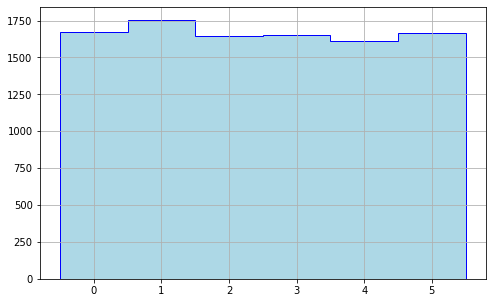
\includegraphics[width=0.7\textwidth]{lesson4_files/lesson4_3_0.png}
\caption{Uniform distribution generated with \texttt{random.randint} function.}
\label{fig:uniform_dist}
\end{figure}
    
Another useful module that we will use later to generate random numbers is \texttt{numpy}, it has similar functionalities as \texttt{random} but in some cases it fits better to our needs.    
Below an example with \texttt{numpy.random.normal} which allows to throw random numbers according to a normal distribution
(\(\mathcal{N}(0, 1)\)), its plot is shown in Fig.~\ref{fig:gauss_dist}.

 \begin{tcolorbox}[breakable, size=fbox, boxrule=1pt, pad at break*=1mm,colback=cellbackground, colframe=cellborder]
\begin{Verbatim}[commandchars=\\\{\}]
\PY{k+kn}{from} \PY{n+nn}{numpy}\PY{n+nn}{.}\PY{n+nn}{random} \PY{k}{import} \PY{n}{normal}
\PY{k+kn}{from} \PY{n+nn}{matplotlib} \PY{k}{import} \PY{n}{pyplot} \PY{k}{as} \PY{n}{plt}

\PY{n}{gauss} \PY{o}{=} \PY{p}{[}\PY{p}{]}
\PY{k}{for} \PY{n}{\PYZus{}} \PY{o+ow}{in} \PY{n+nb}{range}\PY{p}{(}\PY{l+m+mi}{50000}\PY{p}{)}\PY{p}{:}
  \PY{n}{gauss}\PY{o}{.}\PY{n}{append}\PY{p}{(}\PY{n}{normal}\PY{p}{(}\PY{p}{)}\PY{p}{)}
  
\PY{n}{plt}\PY{o}{.}\PY{n}{hist}\PY{p}{(}\PY{n}{gauss}\PY{p}{,} \PY{l+m+mi}{100}\PY{p}{,} \PY{n+nb}{range}\PY{o}{=}\PY{p}{[}\PY{o}{\PYZhy{}}\PY{l+m+mi}{4}\PY{p}{,} \PY{l+m+mi}{4}\PY{p}{]}\PY{p}{)}
\PY{n}{plt}\PY{o}{.}\PY{n}{title}\PY{p}{(}\PY{l+s+s2}{\PYZdq{}}\PY{l+s+s2}{Example of Gaussian distribution from numpy}\PY{l+s+s2}{\PYZdq{}}\PY{p}{)}
\PY{n}{plt}\PY{o}{.}\PY{n}{show}\PY{p}{(}\PY{p}{)}
\end{Verbatim}
\end{tcolorbox}

 \begin{figure}
   \centering
   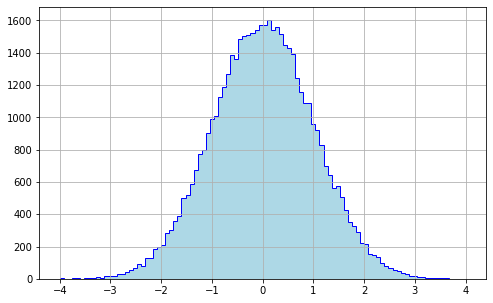
\includegraphics[width=0.7\textwidth]{lesson4_files/lesson4_5_0.png}
   \caption{Normal distribution generated with \texttt{numpy.random.normal} function.}
\label{fig:gaussian_dist}
 \end{figure}

\section{Practical Examples of Monte Carlo
Simulation}\label{example-of-monte-carlo-simulation}

In this Section we go through some applications of the Monte Carlo method.

\subsubsection{Probability to draw two kings from a deck}
Using a frequentist approach, we can calculate the
probability of an event as the ratio of the number of favorable outcomes
of an experiment (number of successes) and the number of all possible
outcomes. 

Imagine we would like to determine the probability of drawing two kings from a standard deck of cards.
At the beginning we have 40 cards (i.e. the entire deck) with 4 possible kings so the probability to get a king is $4/40$. Next, assuming we got a king the first time, we are left with 39 cards and 3 kings only so the probability to get the second king is $3/39$. Since we want both events to happen, the final probability is product of the two contributions:

\[P_\textrm{two kings} = \frac{4}{40} \cdot \frac{3}{39} = \frac{1}{130} \approx 0.0077\]

Let's now try with a Monte Carlo simulation following the steps outlined above and check if we get the same number.
\begin{itemize}
\item \emph{Define a domain of possible inputs}: in this case the domain is a deck of cards. With the \texttt{*} operator a list can be easily repeated many times. In this case it is enough four times, once for each suit (in the example we also set the seed to 1 to make it reproducible).

\begin{tcolorbox}[breakable, size=fbox, boxrule=1pt, pad at break*=1mm,colback=cellbackground, colframe=cellborder]
\begin{Verbatim}[commandchars=\\\{\}]
\PY{k+kn}{from} \PY{n+nn}{random} \PY{k}{import} \PY{n}{sample}\PY{p}{,} \PY{n}{choices}\PY{p}{,} \PY{n}{seed}

\PY{n}{seed}\PY{p}{(}\PY{l+m+mi}{1}\PY{p}{)}

\PY{n}{deck} \PY{o}{=} \PY{p}{[}\PY{l+s+s2}{\PYZdq{}}\PY{l+s+s2}{A}\PY{l+s+s2}{\PYZdq{}}\PY{p}{,} \PY{l+s+s2}{\PYZdq{}}\PY{l+s+s2}{2}\PY{l+s+s2}{\PYZdq{}}\PY{p}{,} \PY{l+s+s2}{\PYZdq{}}\PY{l+s+s2}{3}\PY{l+s+s2}{\PYZdq{}}\PY{p}{,} \PY{l+s+s2}{\PYZdq{}}\PY{l+s+s2}{4}\PY{l+s+s2}{\PYZdq{}}\PY{p}{,} \PY{l+s+s2}{\PYZdq{}}\PY{l+s+s2}{5}\PY{l+s+s2}{\PYZdq{}}\PY{p}{,} \PY{l+s+s2}{\PYZdq{}}\PY{l+s+s2}{6}\PY{l+s+s2}{\PYZdq{}}\PY{p}{,} \PY{l+s+s2}{\PYZdq{}}\PY{l+s+s2}{7}\PY{l+s+s2}{\PYZdq{}}\PY{p}{,} \PY{l+s+s2}{\PYZdq{}}\PY{l+s+s2}{J}\PY{l+s+s2}{\PYZdq{}}\PY{p}{,} \PY{l+s+s2}{\PYZdq{}}\PY{l+s+s2}{Q}\PY{l+s+s2}{\PYZdq{}}\PY{p}{,} \PY{l+s+s2}{\PYZdq{}}\PY{l+s+s2}{K}\PY{l+s+s2}{\PYZdq{}}\PY{p}{]} \PY{o}{*} \PY{l+m+mi}{4}
 \end{Verbatim}
\end{tcolorbox}

\item \emph{Generate inputs randomly from a probability distribution over the defined domain}: which means we draw randomly cards with uniform probability since the deck is fair and all cards have the same probability to be drawn. 
We plan to do 1 million simulations, each time with the \texttt{sample} function we pick up two cards with uniform probability from our virtual deck (for debugging purpose the first 10 trials are printed).

\begin{tcolorbox}[breakable, size=fbox, boxrule=1pt, pad at break*=1mm,colback=cellbackground, colframe=cellborder]
\begin{Verbatim}[commandchars=\\\{\}]
\PY{n}{trials} \PY{o}{=} \PY{l+m+mi}{1000000}
\PY{n}{successes} \PY{o}{=} \PY{l+m+mi}{0}

\PY{k}{for} \PY{n}{i} \PY{o+ow}{in} \PY{n+nb}{range}\PY{p}{(}\PY{n}{trials}\PY{p}{)}\PY{p}{:}
  \PY{n}{cards} \PY{o}{=} \PY{n}{sample}\PY{p}{(}\PY{n}{deck}\PY{p}{,} \PY{n}{k}\PY{o}{=}\PY{l+m+mi}{2}\PY{p}{)}
  \PY{k}{if} \PY{n}{i} \PY{o}{\PYZlt{}} \PY{l+m+mi}{10}\PY{p}{:}
    \PY{n+nb}{print} \PY{p}{(}\PY{n}{cards}\PY{p}{)}
\end{Verbatim}
\end{tcolorbox}

\item \emph{Perform a deterministic computation on the generated inputs}: this step is particularly simple in this case, we just need to check if the draw is \texttt{['K', 'K']} and in case increase the counter of successes.

\begin{tcolorbox}[breakable, size=fbox, boxrule=1pt, pad at break*=1mm,colback=cellbackground, colframe=cellborder]
\begin{Verbatim}[commandchars=\\\{\}]
  \PY{k}{if} \PY{n}{cards} \PY{o}{==} \PY{p}{[}\PY{l+s+s2}{\PYZdq{}}\PY{l+s+s2}{K}\PY{l+s+s2}{\PYZdq{}}\PY{p}{,} \PY{l+s+s2}{\PYZdq{}}\PY{l+s+s2}{K}\PY{l+s+s2}{\PYZdq{}}\PY{p}{]}\PY{p}{:}
    \PY{n}{successes} \PY{o}{+}\PY{o}{=} \PY{l+m+mi}{1}
 \end{Verbatim}
\end{tcolorbox}

\item \emph{Aggregate the results}: finally we just print successes/trials which is the sought probability.

\begin{tcolorbox}[breakable, size=fbox, boxrule=1pt, pad at break*=1mm,colback=cellbackground, colframe=cellborder]
\begin{Verbatim}[commandchars=\\\{\}]
\PY{n+nb}{print} \PY{p}{(}\PY{l+s+s2}{\PYZdq{}}\PY{l+s+s2}{The probability to draw two kings is }\PY{l+s+si}{\PYZob{}:.4f\PYZcb{}}\PY{l+s+s2}{\PYZdq{}}\PY{o}{.}\PY{n}{format}\PY{p}{(}\PY{n}{successes}\PY{o}{/}\PY{n}{trials}\PY{p}{)}\PY{p}{)}

['Q', '7']
['5', '7']
['J', '2']
['Q', 'A']
['5', '4']
['7', '2']
['2', '5']
['J', 'Q']
['A', 'Q']
['J', '5']
The probability to draw two kings is 0.0077
    \end{Verbatim}
\end{tcolorbox}
\end{itemize}
The result is in agreement with our theoretical expectations.

\subsubsection{Dice probabilities}
Two fair dice are rolled, find the probability that their sum is:
\begin{enumerate}
\item equal to 1
\item equal to 4
\item less than 13
\end{enumerate}

Before looking at the \texttt{python} implementation let's compute what we should get: the possible combinations
of the outcomes of two dice are 36 (to realize it you can simply think that for each one of the six faces of the first die you have six possible faces of the second hence $6\cdot 6=35$). It is not possible to get 1 since
the dice have no face with 0 so the first probability should come out 0. The sum of the two dice is always less than 13 
(the maximum is 12\ldots) so the answer to point 3 is 1. We can get a sum of 4 in 3 cases (1-3, 3-1 or 2-2) so the expected probability is $3/36=1/12=0.0833$

Implement again the steps of Monte Carlo simulation, now throwing two random integers (with \texttt{randint}) to simulate the dice, and count how many times their sum is 0, 4 and lower than 13.

\begin{tcolorbox}[breakable, size=fbox, boxrule=1pt, pad at break*=1mm,colback=cellbackground, colframe=cellborder]
\begin{Verbatim}[commandchars=\\\{\}]
\PY{k+kn}{import} \PY{n+nn}{random}

\PY{n}{random}\PY{o}{.}\PY{n}{seed}\PY{p}{(}\PY{l+m+mi}{1}\PY{p}{)}

\PY{n}{successes} \PY{o}{=} \PY{p}{\PYZob{}}\PY{l+s+s2}{\PYZdq{}}\PY{l+s+s2}{=0}\PY{l+s+s2}{\PYZdq{}}\PY{p}{:}\PY{l+m+mf}{0.0}\PY{p}{,} \PY{l+s+s2}{\PYZdq{}}\PY{l+s+s2}{=4}\PY{l+s+s2}{\PYZdq{}}\PY{p}{:}\PY{l+m+mf}{0.0}\PY{p}{,} \PY{l+s+s2}{\PYZdq{}}\PY{l+s+s2}{\PYZlt{}13}\PY{l+s+s2}{\PYZdq{}}\PY{p}{:}\PY{l+m+mf}{0.0}\PY{p}{\PYZcb{}}
\PY{n}{trials} \PY{o}{=} \PY{l+m+mi}{100000}
\PY{k}{for} \PY{n}{\PYZus{}} \PY{o+ow}{in} \PY{n+nb}{range}\PY{p}{(}\PY{n}{trials}\PY{p}{)}\PY{p}{:}
    \PY{n}{d1} \PY{o}{=} \PY{n}{random}\PY{o}{.}\PY{n}{randint}\PY{p}{(}\PY{l+m+mi}{1}\PY{p}{,} \PY{l+m+mi}{6}\PY{p}{)}
    \PY{n}{d2} \PY{o}{=} \PY{n}{random}\PY{o}{.}\PY{n}{randint}\PY{p}{(}\PY{l+m+mi}{1}\PY{p}{,} \PY{l+m+mi}{6}\PY{p}{)}
    \PY{k}{if} \PY{p}{(}\PY{n}{d1} \PY{o}{+} \PY{n}{d2}\PY{p}{)} \PY{o}{==} \PY{l+m+mi}{0}\PY{p}{:}
        \PY{n}{successes}\PY{p}{[}\PY{l+s+s2}{\PYZdq{}}\PY{l+s+s2}{=0}\PY{l+s+s2}{\PYZdq{}}\PY{p}{]} \PY{o}{+}\PY{o}{=} \PY{l+m+mf}{1.0}
    \PY{k}{if} \PY{p}{(}\PY{n}{d1} \PY{o}{+} \PY{n}{d2}\PY{p}{)} \PY{o}{==} \PY{l+m+mi}{4}\PY{p}{:}
        \PY{n}{successes}\PY{p}{[}\PY{l+s+s2}{\PYZdq{}}\PY{l+s+s2}{=4}\PY{l+s+s2}{\PYZdq{}}\PY{p}{]} \PY{o}{+}\PY{o}{=} \PY{l+m+mf}{1.0}
    \PY{k}{if} \PY{p}{(}\PY{n}{d1} \PY{o}{+} \PY{n}{d2}\PY{p}{)} \PY{o}{\PYZlt{}} \PY{l+m+mi}{13}\PY{p}{:}
        \PY{n}{successes}\PY{p}{[}\PY{l+s+s2}{\PYZdq{}}\PY{l+s+s2}{\PYZlt{}13}\PY{l+s+s2}{\PYZdq{}}\PY{p}{]} \PY{o}{+}\PY{o}{=} \PY{l+m+mf}{1.0}
    
\PY{k}{for} \PY{n}{k}\PY{p}{,}\PY{n}{v} \PY{o+ow}{in} \PY{n}{successes}\PY{o}{.}\PY{n}{items}\PY{p}{(}\PY{p}{)}\PY{p}{:}
    \PY{n+nb}{print} \PY{p}{(}\PY{l+s+s2}{\PYZdq{}}\PY{l+s+s2}{P(}\PY{l+s+si}{\PYZob{}\PYZcb{}}\PY{l+s+s2}{): }\PY{l+s+si}{\PYZob{}:.3f\PYZcb{}}\PY{l+s+s2}{\PYZdq{}}\PY{o}{.}\PY{n}{format}\PY{p}{(}\PY{n}{k}\PY{p}{,} \PY{n}{v}\PY{o}{/}\PY{n}{trials}\PY{p}{)}\PY{p}{)}

P(=0): 0.000
P(=4): 0.084
P(<13): 1.000
\end{Verbatim}
\end{tcolorbox}

Again the results are very close to our expectations.

\subsection{Accuracy of Monte Carlo Simulation}

Since we rely on a frequentist approach naively we can say that the lower is the probability we need to estimate the higher has to be the number of simulated trials. This is because to get a reasonable number of "success" (to keep the uncertainty in the probability small), we have to try many times. This is apparent playing with the number of trials in the above simulations. 

This is also the main reason why, despite its undoubted power, Monte Carlo simulation is not always the best approach to follow.
Many times indeed the simulation of an experiment requires a lot of computing resources (and time) and it may not be practical to embark into such a large simulation.

To quantify the error associated to a Monte Carlo estimate remember that our estimate of the true value $\hat{\mu}_n$ is itself a random variable (like $Y$) with its mean and variance. We know that the best approximation of the true value is:

\[\mathbb{E}(\hat{\mu}_n) = \frac{1}{n}\sum_{i=1}^{n}\mathbb{E}(Y_i)=\mu \]
and the root mean squared error is 
\[\mathrm{RMSE} = \sqrt{\mathbb{E}((\hat{\mu}_n - \mu)^2)}=\sqrt{\cfrac{\sigma^2}{n}} = \cfrac{\sigma}{\sqrt{n}}\]
where $\sigma^2 = \mathrm{Var}(Y)$.

While it is obvious that the estimate should get worse with increased variance and better with increased sample size, this equation  gives us the exact rate of exchange. 

The RMSE tells us that to get one more decimal digit of accuracy (i.e. an RMSE one tenth as large) requires a 100-fold increase in computation. To get three more digits of accuracy requires one million times as much computation. From that it is clear that simple Monte Carlo computation is poorly suited for problems that must be answered with high precision.

On the other hand if raising $n$ from $n_1$ to $n_2$ only makes our accuracy a little better, then reducing $n$ from $n_2$ to $n_1$ must only make our accuracy a little worse. Then we might well decide that for software (i.e. experiment) that runs slower, is worthwhile reducing $n$ if it provides some other benefit, such as a more rapid programming.

\subsection{Derivation of log-normal Stochastic Differential
Equation}\label{derivation-of-log-normal-stochastic-differential-equation}

In this Section we try to see how to implement the simulation of a stock price which deviates from a steady state as a result of random fluctuations given by the trades. 

Considering a stock with a price \(S_t\) and an expected rate of return \(\mu\); the relative change in its price during a period \(dt\) can be decomposed in two parts:

\begin{itemize}
\tightlist
\item
  a deterministic part that is the expected return from the stock held
  during the time period \(dt\) and which can be expressed as \(\mu S_tdt\)
\item
  a stochastic part which reflects the random changes of the market
  (e.g. as a response to external effects such as unexpected news). A
  reasonable assumption is to take this contribution proportional to the
  stock so \(\sigma S_t dB_t\), where \(dB_t\) is a so called random walk process equal to \(\epsilon\sqrt{t}=\mathcal{N}(0,1)\sqrt{t}\).
\end{itemize}
Putting the two contribution together the resulting differential equation is:

\begin{equation}
  dS_t = \mu S_tdt + \sigma S_tdB_t
  \label{eq:differential}
\end{equation}
or dividing by $S_t$
\[\frac{dS_t}{S_t} = d\textrm{log}(S_t) = \mu dt + \sigma dB_t\]

    The solution of this equation can be derived by applying the
It\(\hat{o}\)'s formula which states that for any given function
\(G(S, t)\) where \(S\) satisfies the following stochastic differential
equation \(dS=a\cdot dt +b\cdot dB_t\) it holds:

\begin{equation}
dG=\big(a\frac{\partial G}{\partial S} + \frac{\partial G}{\partial t} + \frac{1}{2}b^2\frac{\partial^2 G}{\partial S^2} \big)dt + b \frac{\partial G}{\partial S}dB
\label{eq:itos_lemma}
\end{equation}

Now if we set \(G = \textrm{log}(S_t)\) we can compute the derivatives:

\[\frac{\partial G}{\partial S} = \frac{1}{S_t}\]

\[\frac{\partial G}{\partial t} = 0\]

\[\frac{\partial^2 G}{\partial S^2} = -\frac{1}{S_t^{2}}\]

Substituting back into Eq.~\ref{eq:itos_lemma} and taking the values of $a$ and $b$ from Eq.~\ref{eq:differential} we get:

\[d(\textrm{log} S_t) = \big(\mu S_t \cfrac{1}{S_t} + \cfrac{1}{2}\sigma^2 S_t^2 (-\cfrac{1}{S_t^2})\big)dt + \sigma\epsilon\sqrt{dt}\]

\[d(\textrm{log} S_t) = \textrm{log} (S_t) - \textrm{log} (S_{t-1}) = \textrm{log} \cfrac{S_t}{S_{t-1}} = \big(\mu - \cfrac{1}{2}\sigma^2\big)dt + \sigma\epsilon\sqrt{dt}\]

\[S_t = S_{t-1}e^{\big(\mu - \cfrac{1}{2}\sigma^2\big)dt + \sigma\epsilon\sqrt{dt}}\]

As can be seen from the following equation:

\[d(\textrm{log} S_t) = \big(\mu - \cfrac{1}{2}\sigma^2\big)dt + \sigma\epsilon\sqrt{dt}\]
the change in \(\textrm{log} S_t\) has a constant \emph{drift} with respect to time 
\(\mu - \frac{1}{2}\sigma^2\) and a constant variance rate \(\sigma^2\)
(remember that \(\epsilon\) is a normally distributed random variable
\(\mathcal{N}(0,1)\)). So you have a constant plus a Gaussian
distributed variable, therefore \(\textrm{log} S_t\) at some time \(T\)
is normally distributed with:

\[\textrm{log}S_t - \textrm{log}S_0 \approx\mathcal{N}\big[\big(\mu-\frac{\sigma^2}{2}\big)T, \sigma^2 T\big]\]

This equation shows that \(\textrm{log}S_t\) is normally distributed,
but \textbf{a variable whose logarithm is normally distributed is said
to be log-normal}. The model we have just developed implies that
the stock price at time T, given today's price, is log-normally
distributed. One of the nicer property of a log-normal distribution is to be positive defined and that's why log-normality is an important characteristic: we need to \emph{ensure} that a stock price will never be negative. Actually this result was expected, in fact looking at the initial \(dS\) equation (Eq.~\ref{eq:differential}) we had:

\[dS_t = \mu S_tdt + \sigma S_tdB_t\]
which shows that the closer \(S_t\) is to 0, the smaller is its variation \(dS\), so it will never go negative.

Let's then implement the simulation of a stock price.

\begin{tcolorbox}[breakable, size=fbox, boxrule=1pt, pad at break*=1mm,colback=cellbackground, colframe=cellborder]
\begin{Verbatim}[commandchars=\\\{\}]
\PY{k+kn}{from} \PY{n+nn}{numpy}\PY{n+nn}{.}\PY{n+nn}{random} \PY{k}{import} \PY{n}{normal}\PY{p}{,} \PY{n}{seed} 
\PY{k+kn}{from} \PY{n+nn}{matplotlib} \PY{k}{import} \PY{n}{pyplot} \PY{k}{as} \PY{n}{plt} 
\PY{k+kn}{import} \PY{n+nn}{math}
		
\PY{c+c1}{\PYZsh{}initial price}
\PY{n}{S} \PY{o}{=} \PY{l+m+mi}{100}
\PY{n}{mu} \PY{o}{=} \PY{o}{\PYZhy{}}\PY{l+m+mf}{0.01} 
\PY{n}{sigma} \PY{o}{=} \PY{l+m+mf}{0.05} 
\PY{n}{T}\PY{o}{=}\PY{l+m+mi}{1}
\PY{n}{seed}\PY{p}{(}\PY{l+m+mi}{1}\PY{p}{)} 
\PY{n}{historical\PYZus{}series} \PY{o}{=} \PY{p}{[}\PY{n}{S0}\PY{p}{]}
\PY{c+c1}{\PYZsh{} 30 days simulation}
\PY{k}{for} \PY{n}{i} \PY{o+ow}{in} \PY{n+nb}{range}\PY{p}{(}\PY{l+m+mi}{30}\PY{p}{)}\PY{p}{:}
    \PY{n}{S} \PY{o}{=} \PY{n}{S} \PY{o}{*} \PY{n}{math}\PY{o}{.}\PY{n}{exp}\PY{p}{(}\PY{p}{(}\PY{n}{mu} \PY{o}{\PYZhy{}} \PY{l+m+mf}{0.5} \PY{o}{*} \PY{n}{sigma} \PY{o}{*} \PY{n}{sigma}\PY{p}{)} \PY{o}{*} \PY{n}{T} \PY{o}{+}
    \PY{n}{sigma} \PY{o}{*} \PY{n}{math}\PY{o}{.}\PY{n}{sqrt}\PY{p}{(}\PY{n}{T}\PY{p}{)} \PY{o}{*} \PY{n}{normal}\PY{p}{(}\PY{p}{)}\PY{p}{)}
    \PY{n}{historical\PYZus{}series}\PY{o}{.}\PY{n}{append}\PY{p}{(}\PY{n}{S}\PY{p}{)}
\end{Verbatim}
\end{tcolorbox}
The result of the simulation is shown in Fig.~\ref{fig:stock_price_sim}.

\begin{figure}[htb]
	\centering
	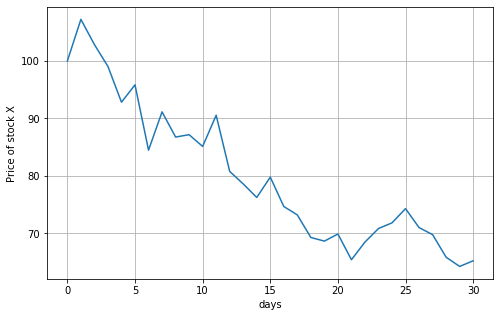
\includegraphics[width=0.7\textwidth]{lesson4_files/lesson4_12_0.png}
	\caption{Simulation with Monte Carlo method of a stock price, using the log-normal evolution.}
	\label{fig:stock_price_sim}
\end{figure}


